% Kapitel 3

\chapter{Data Efficiency in Neural Network-Based Image Segmentation}
\label{chap:data-efficiency}

Above all, the accuracy of neural networks is governed by three factors: problem complexity, model complexity, and the sample size. Each of these factors contribute to accuracy in different ways and they have complex interdependent relationships. Grasping the concept of data efficiency necessitates an understanding of these three aspects. In this chapter, we will elucidate how the three factors impact model error by examining neural networks as function approximators.

Consider a machine learning scenario where we estimate the 10-year risk of heart disease based on age. However, we don't know the underlying function, Our only recourse is to gather data points and strive to approximate this hidden function. Essentially, our goal is to discover a function that minimizes a criterion, which measures the discrepancy between the theoretical curve and our collected data points.

Consider a machine learning scenario where we estimate the 10-year risk of heart disease based on age. Here, some underlying function maps age to heart disease risk. However, there is no way to know what this function is. Our only recourse is to collect a set of data points and try to approximate the underlying function. Essentially, our goal is to find a function by minimizing some criterion which measures the error between the function and our collected data points.

Given any number of points, one can construct an infinite number of functions that fit those points equally well under a selected criterion. Therefore, to derive a single solution, we have to choose a finite class of functions to evaluate. One of the simplest classes of functions we could use are lines -- leading to a simple linear regression. A line is defined by two parameters, its slope $\theta_1$ and intersect $\theta_0$:

\begin{equation}
	f(x) = \theta_1 x + \theta_0
\end{equation}

In this equation, $f(x)$ represents our regression model. The objective is to determine the optimal value of $\theta = \{ \theta_1, \theta_2 \}$ that most accurately represent the collected data pairs $(x_i, y_i)$. This can be achieved by minimizing the mean squared distance between the line and each data point:

\begin{equation}
	\min_{\theta} \sum_{i=1}^N (y_i - f(x_i))^2.
\end{equation}

We will conduct a simulated experiment where our underlying function is a cosine function, with each point sampled having additive Gaussian noise:

\begin{equation}
	y(x) = -(\cos(0.01 \pi x) - 1) \cdot 0.4 + Z, Z \sim \mathcal{N}(0, 0.1).
\end{equation}

We'll generate several $(x_i, y_i)$ pairs and apply the previously discussed linear model and criterion to fit a line through these points. In real world conditions, the underlying function and the nature of the measurement noise remain unknown. However, for this simulation, knowing these details is useful to demonstrate the divergence between the fitted function and the underlying one. Figure \ref{fig:t1-t2-example} illustrates the fitted line using varying numbers of data points.

\begin{figure}[h!]
 \hfill
 \subfloat{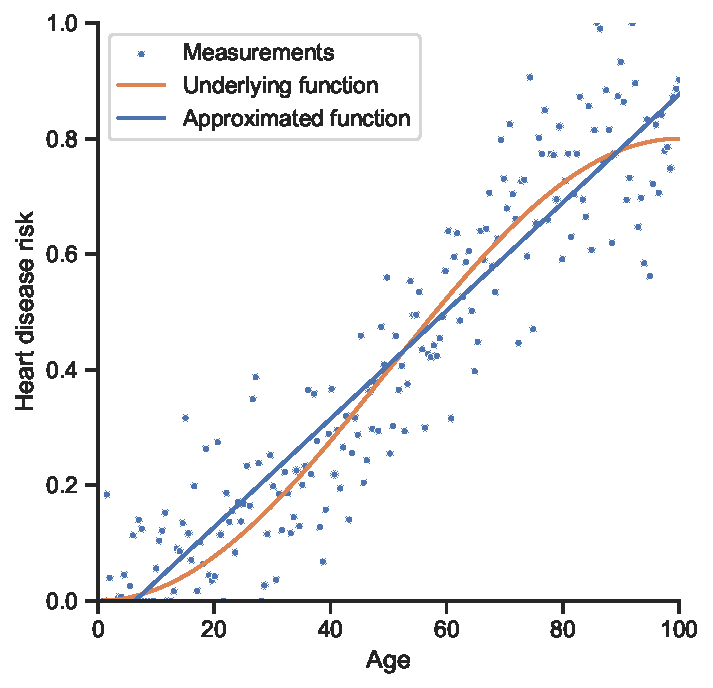
\includegraphics[width=0.5\linewidth]{images/3/heart_disease_risk}}
 \hfill
 \subfloat{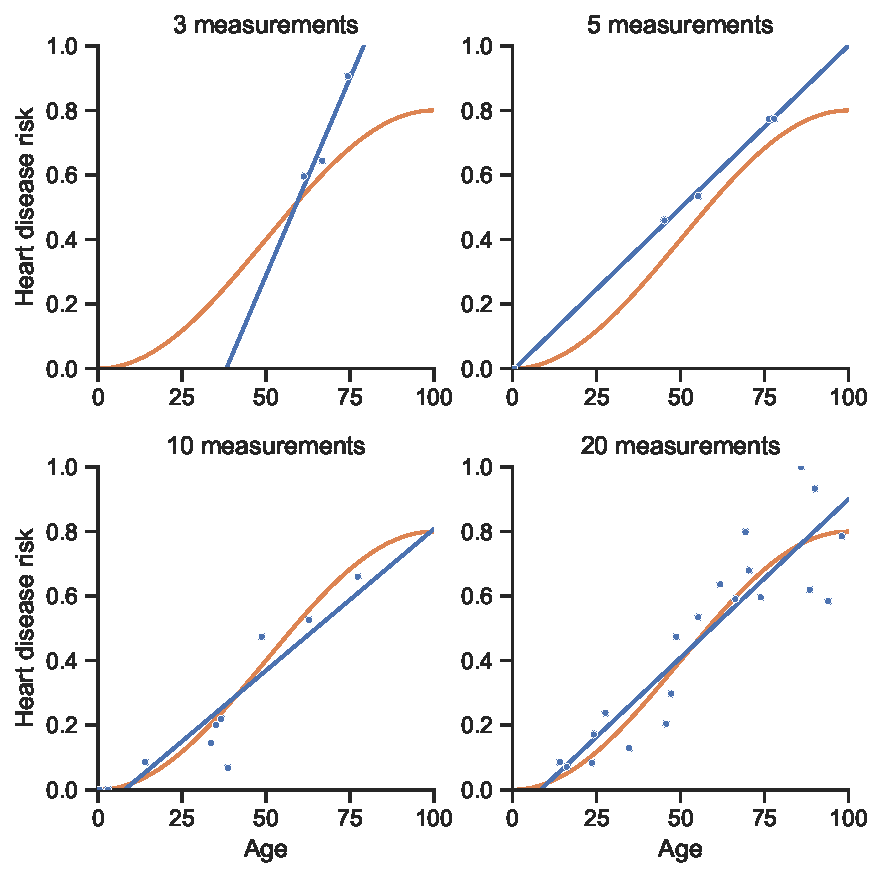
\includegraphics[width=0.5\linewidth]{images/3/heart_disease_risk_samples}}
 \hfill
 \caption{A simulated example of heart disease risk prediction using simple linear regression. The plots on the right show how the approximated function depends on the sample size.\label{fig:t1-t2-example}}
\end{figure}

The simulation with only three points clearly demonstrates a mismatch between the approximated and underlying functions. This discrepancy is known as \textbf{overfitting}. Overfitting occurs when the model is overly influenced by the specific sample of data, particularly the noise, and fails to generalize to new, unseen examples. As the number of samples increases, the approximated function aligns more closely with the underlying one. However, even with 20 measurements, there is a notable difference between the approximated and underlying functions. The underlying function is a non-linear cosine function. No matter how many data points we use, a model with only two parameters cannot perfectly approximate this non-linear function. This is an example of \textbf{underfitting}, where the model lacks sufficient parameters to capture the complexity of the underlying function.

To address underfitting, a more complex model is required, meaning we need a broader class of functions for optimization. Our current regression can be viewed as fitting a polynomial function to the dataset. Initially, we have employed polynomials of degree 1 — lines. We can generalize our model to an $n$-degree polynomial:

\begin{equation}
	f(x) = \theta_n x^n + \theta_{n-1}x^{n-1} + \cdots + \theta_1 x + \theta_0.
\end{equation}

To increase our function class, we will choose a larger polynomial degree and again minimize the mean squared distance to obtain $\theta_n$ through $\theta_0$. By increasing the degree we are increasing the complexity of the model and the model will be able to represent more complex underlying functions. We can observe what happens when we choose degrees 2, 3, or 5 in \figref{fig:reg-deg-2}.

\begin{figure}[h!]
 \centering
 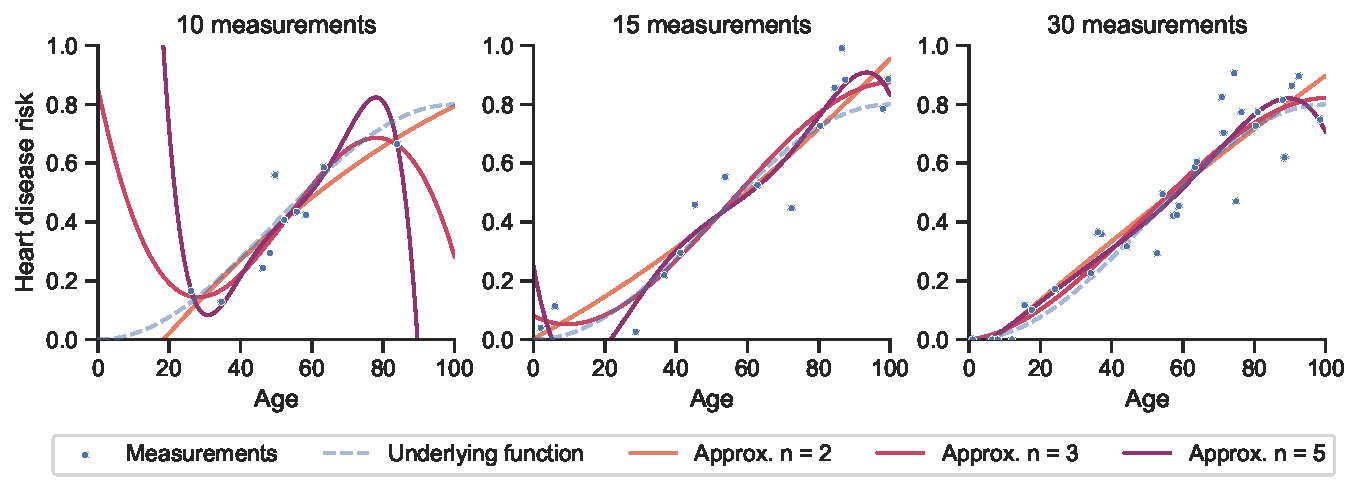
\includegraphics[width=\linewidth]{images/3/heart_disease_risk_samples_degrees}
 \caption{Fitting a polygonal function of various degrees on three different sample sizes.}
 \label{fig:reg-deg-2}
\end{figure}

In the case with 10 measurements, we observe that the approximated polynomial with $n = 2$ follows the underlying function somewhat well. However, as we increase the degree the function quickly begins to overfit. This experiment demonstrates that the likelihood of overfitting escalates with increased model complexity. Yet, we need complex models to approximate complex functions.

The inherent conflict between overfitting and underfitting is known as the \textbf{bias--complexity tradeoff} (alternatively, the bias–variance tradeoff). Let us investigate this problem more formally. We can decompose the error of a deep learning model into two components \cite{shalev-shwartzUnderstandingMachineLearning2014}. Consider a trained model $f_\theta$ with optimal parameter values $\theta$ from a class of functions $\mathcal{F}$. Let there be a function $L(f)$ that measures the error between any model $f \in \mathcal{F}$ and the underlying function we are approximating. The total error of the trained model can be expressed as:

\begin{equation}
	L(f_\theta) = \epsilon_{app} + \epsilon_{est}
	\text{ where:\;}  \epsilon_{app} = \min_{f \in F}L(f),\;
	\epsilon_{est} = L(f_\theta) - \epsilon_{app},
\end{equation}

where $\epsilon_{app}$ is the \textbf{approximation error} and $\epsilon_{est}$ is the \textbf{estimation error}. The approximation error is the residual error when using the best possible approximator within our chosen class of functions $F$. For instance, in the earlier function approximation example with a 1st-degree polynomial, even with infinite data, there would always be some discrepancy in approximation compared to the underlying function. The approximation error solely depends entirely on the class of functions we use and can only be reduced by adopting a different class, such as polynomials of a higher degree. The remaining estimation error depends on the quality of our parameters $\theta$. It is possible to have a class of functions capable of perfectly approximating the underlying function but still fail to precisely identify the optimal function within that class.

In our previous experiment, we observed that the estimation error is influenced by both the sample size and the complexity of the model. To formally analyze this, we can explore the concept of \textbf{sample complexity}. Sample complexity, denoted as $n(\epsilon, \delta)$ for chosen $\epsilon, \delta \in (0, 1)$ measures the number of samples needed for a model $f$ chosen from a finite class of functions $\mathcal{F}$ to be \textbf{probably approximately correct}. This means that, across different samplings of data points, there is a probability of $1 - \delta$ that the model is correct within some margin of error $\epsilon$, i.e. $L(f) \leq \epsilon$. Assuming there exists some unknown $f' \in F$ for which $L(f') = 0$, it can be shown \cite{shalev-shwartzUnderstandingMachineLearning2014} that:

\begin{equation}
	n(\epsilon, \delta) \geq \frac{\log(\lvert F \rvert \delta)}{\epsilon}.
\end{equation}

We can see that increasing the function class $\lvert \mathcal{F} \rvert$ necessitates a larger sample size $n$ to probably approximately correctly approximate the underlying function. Thus, we conclude that the estimation error can be reduced either by adding more data samples or by decreasing the size of the function class we are optimizing over.

In medical image segmentation we have an unfortunate stalemate between the three factors governing estimation and approximation errors. The complexity of medical image segmentation demands a large number of parameters, which in turn increases the estimation error. Ideally, this error could be mitigated by adding more data samples, but in the realm of medical imaging, acquiring ample data is often impractical.

To reduce the estimation error, we are left with reducing the size of the function class. We can do so in two ways. The first involves reducing the parameters of the model itself, shrinking the class of functions and allowing the model to more easily find the optimal function. This usually requires transforming the data such that it can be easily segmented with a less complex model. The second method involves initializing the model with parameters that are already near-optimal. In this case, the model starts close to the optimal function, needing only to search within a local space around these parameters. This is typically achieved by first optimizing the model on similar data for a related task that involves learning features pertinent to segmentation, followed by further optimization for the specific segmentation task.

In the subsequent sections, we will delve into specific techniques from these two approaches, providing examples of their application in neural network-based medical image segmentation.

\section{Transfer Learning}

For example, consider the task of segmenting liver tumors in CT scans. Suppose we have a limited dataset of labeled liver tumor regions, but a more extensive collection of labeled liver regions. In such a scenario, the first step would be to train a neural network for liver segmentation. The rationale here is that most of the parameters learned for liver segmentation will be relevant and close to those needed for liver tumor segmentation. Therefore, when we are developing the liver tumor segmentation network, we copy the values of the parameters learned in the liver segmentation network. We can then say that the network was \textbf{pre-trained} or \textbf{initialized} on a liver segmentation dataset and \textbf{fine-tuned} on the liver tumor segmentation dataset.

In this thesis, we refer to this basic technique as ``simple transfer learning''. There are many other more complex ways of achieving pre-training and fine tuning. In this section, we will present an overview of some of these methods.

	\subsection{Simple Transfer Learning}
	
	Simple transfer learning is a prevalent technique in medical image segmentation. Typically, segmentation neural networks in this field are initialized with weights trained on the ImageNet dataset \cite{dengImageNetLargescaleHierarchical2009a}. ImageNet comprises a collection of natural images, which significantly differ in distribution from medical images. As a result, initializing with ImageNet-trained weights doesn't usually enhance accuracy directly in medical image tasks. However, it aids in expediting the network's convergence. This is because such initialization 'skips' the phase of learning fundamental image features that are common across various types of images, including medical ones. Figure \ref{fig:stl-diagram} illustrates this process.
	
Simple transfer learning is used extensively in medical image segmentation. Segmentation neural networks are commonly initialized using weights trained on the ImageNet dataset \cite{dengImageNetLargescaleHierarchical2009a}. ImageNet is a dataset of natural images and its distribution is drastically different from medical images. Therefore, this initialization does not typically lead to increases in accuracy, but can make the network converge faster as it ``skips'' having to learn to detect base-level image features common to all images. This process is shown in \figref{fig:stl-diagram}.

\begin{figure}[h!]
 \centering
 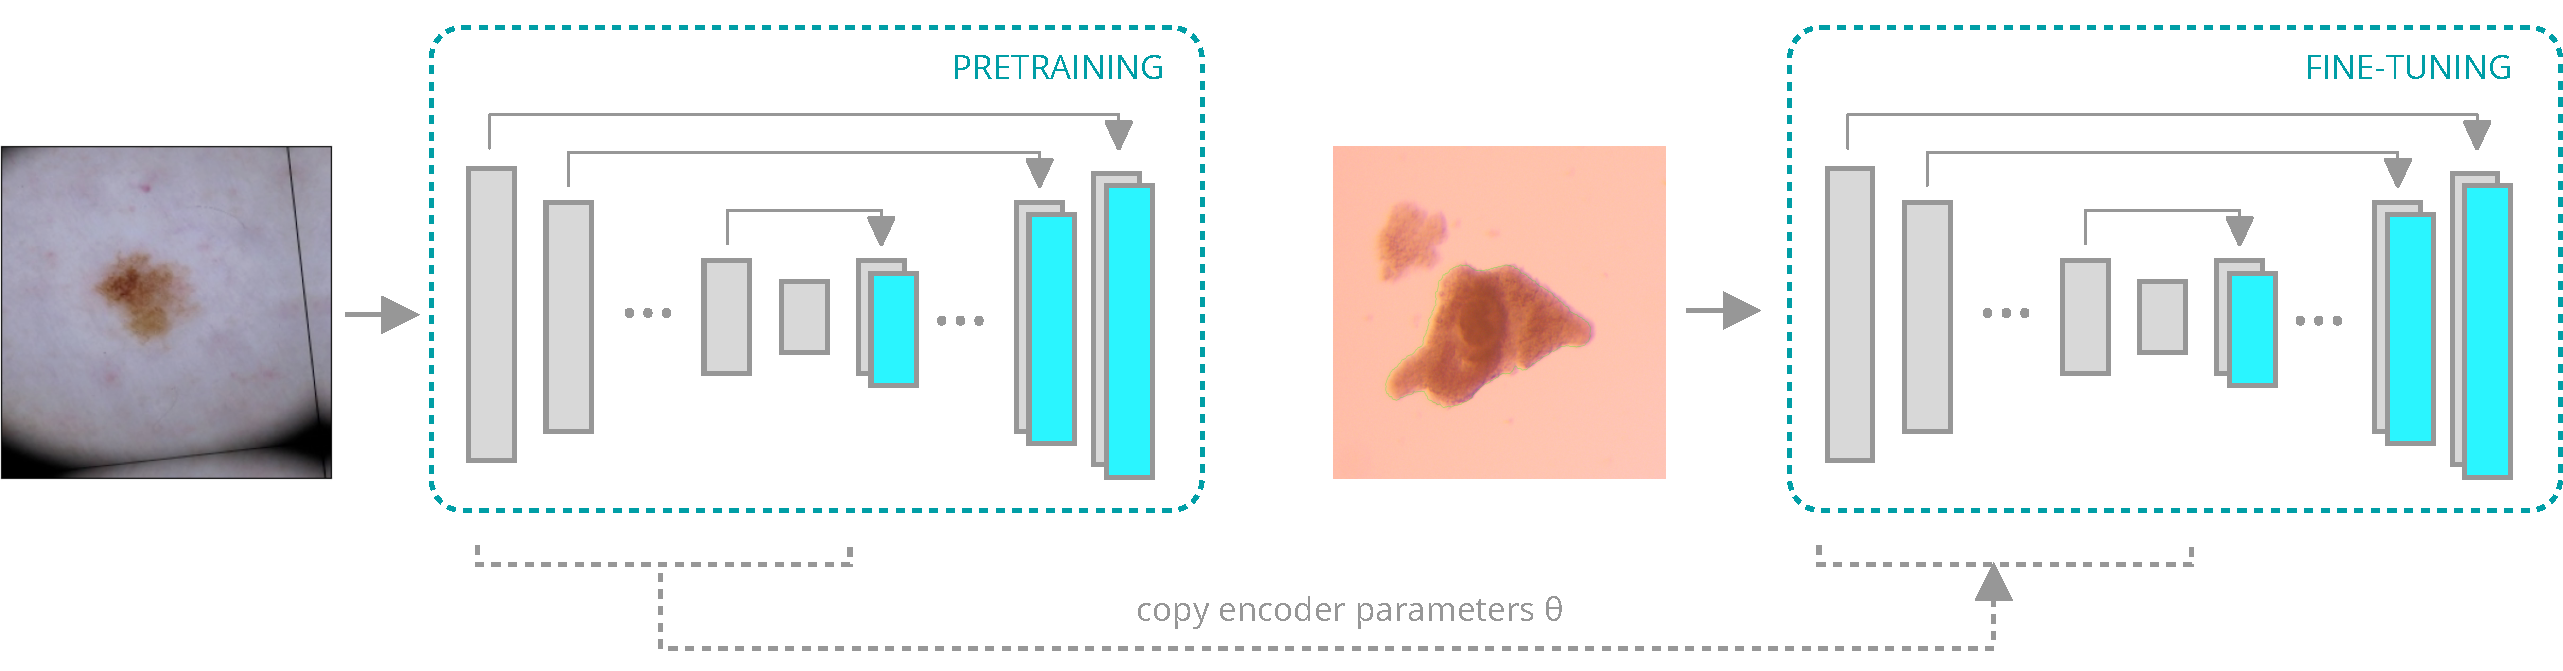
\includegraphics[width=\linewidth]{images/3/simple-transfer-learning-diagram}
 \caption{An overview of the simple transfer learning procedure. First, a model is pretrained on some related segmentation task. Then, part of the trained model's weights are copied to a new model that is then fine-tuned on the target segmentation task.}
 \label{fig:stl-diagram}
\end{figure}

Recent datasets, like those referenced in \cite{wasserthalTotalSegmentatorRobustSegmentation2023}, comprising over 1000 subjects, are increasingly utilized for transfer learning, improving the accuracy of downstream tasks \cite{monaiconsortiumMONAIMedicalOpen2023, myronenkoAutomated3DSegmentation2023}. While these approaches can result in impressive performance improvements, their application is constrained to fields where ample, similar data is accessible. In more specialized modalities or segmentation problems, the knowledge learned during pre-training may not be adequate for improving downstream accuracy.  A potential solution to bridge this gap involves adapting the pre-trained model to the specific target domain, a topic we'll explore in the following section.

	\subsection{Domain Adaptation}
	
Neural networks often struggle to generalize across different datasets, even within similar domains \cite{torralbaUnbiasedLookDataset2011}. This is referred to as the ``domain shift'' problem. Overcoming this problem could lead to an increase in data efficiency, since a model trained on some similar large dataset can perform well on a smaller target dataset. Various domain adaptation techniques have been developed to tackle this challenge.

One class of methods aims to explicitly penalize domain shift by including an estimate of domain shift in the loss function. For instance, \citet{liuUnsupervisedDeepDomain2018} first train a network on a source domain with abundant data. This network is then adapted to perform segmentation on a target domain with limited data. During adaptation, the loss function includes a term for maximum mean discrepancy between the encoded feature vectors of the source and target domains. Minimizing this discrepancy forces the encoder to maintain consistent feature representations rather than shifting the distribution of the encoded feature maps.

Another approach involves reducing the network's ability to distinguish between source and target domains, thereby removing information that leads to domain shift. \citet{ganinDA2015} add a classification head to the network to identify the input's domain. Typically, networks adjust their parameters to minimize loss during each iteration. However, in \cite{ganinDA2015}, the gradients from the domain classifier are inverted so the network updates its parameters to make it harder to differentiate between the two datasets. This method is illustrated in \figref{fig:unsup-dom-adpt}.

\begin{figure}[h!]
 \centering
 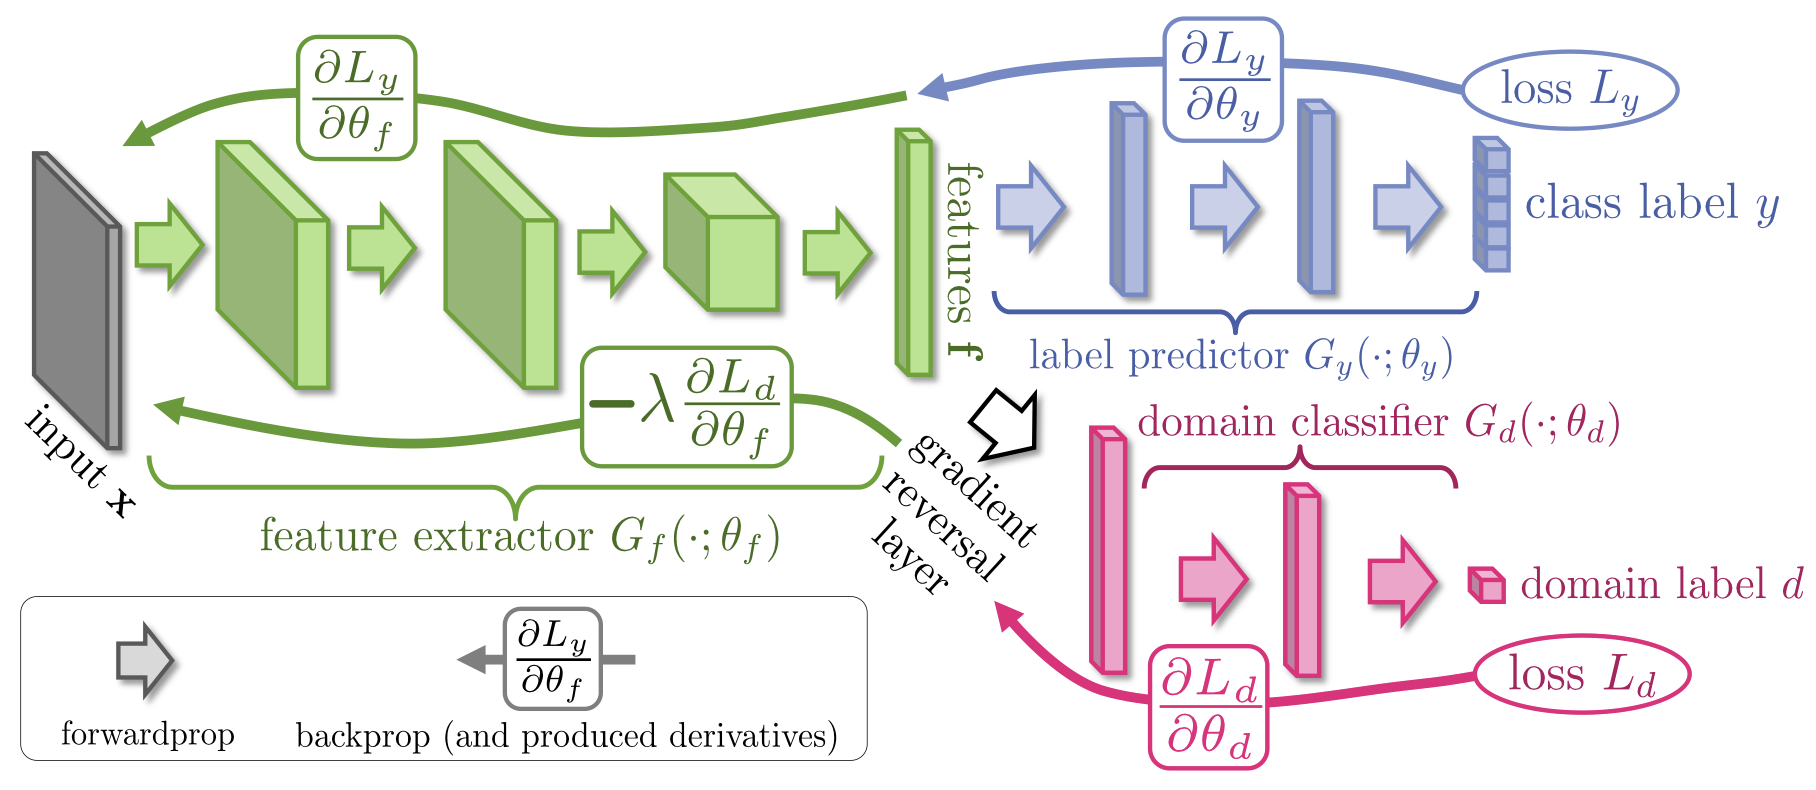
\includegraphics[width=0.7\linewidth]{images/3/unsup-dom-adpt}
 \caption{A diagram of the domain adaptation approach in \citet{ganinDA2015}. The gradients of the domain classification head which are applied to the encoder are reversed during backpropagation.}
 \label{fig:unsup-dom-adpt}
\end{figure}
	
Domain adaptation has been effectively applied to medical image segmentation, as demonstrated in the work of \citet{bermudez-chaconDomainadaptiveTwostreamUNet2018}. They utilized a U-Net-like architecture with dual encoder branches, each processing images from a different domain, paired with a shared decoder. Their loss function incorporates a maximum mean discrepancy term, comparing the decoder’s final feature maps from inputs of both domains. This method was employed for segmenting mitochondria and synapses in microscopic images.

Although domain adaptation techniques enhance transfer learning performance, they generally require labeled data from the source domain. There is growing interest in methods that can utilize unlabeled data to identify general features in images from the target domain regardless of the specific task to be achieved. We'll explore these methods in the following section.

	\subsection{Semi-Supervised and Self-Supervised Learning}
	
Semi-supervised learning combines both labeled and unlabeled data to train neural networks. One such approach is \textbf{self-supervised learning}, where a feature extractor can be trained in a completely unsupervised manner using a large number of images. Then, that feature extractor can employed via transfer learning to train a network for some specific task such as segmentation. Self-supervised learning has
been shown to improve data efficiency
\cite{chenSimpleFrameworkContrastive2020}. 


Various methods exist for training the encoder to learn useful features. One common strategy involves a \textbf{pretext task}, where the network is trained on a task for which solutions can be automatically generated from unlabeled data, allowing for supervised training. An example is provided by \citet{norooziUnsupervisedLearningVisual2016}, where the network is trained to solve a jigsaw puzzle created from an unlabeled dataset. An image is divided into 
3
×
3
3×3 tiles, shuffled, and then fed into the network, which is tasked with reordering these tiles to reconstruct the original image. This process compels the network to learn various image features, as illustrated in \figref{fig:ssl-pretext}.

One common strategy involves a \textbf{pretext task}, where the network is trained on a task for which solutions can be automatically generated from unlabeled data, using automatically generated labels to train the network. A pretext task could be, for instance, solving jigsaw puzzles \cite{norooziUnsupervisedLearningVisual2016}. An image is divided into $3 \times 3$ tiles, the tiles are randomly shuffled and fed into the network, which is tasked with reordering these tiles to reconstruct the original image. By solving this task, the network is forced to learn features such as recognizing a single object across multiple tiles. Such an approach is visualized in \figref{fig:ssl-pretext}.

\begin{figure}[h!]
 \centering
 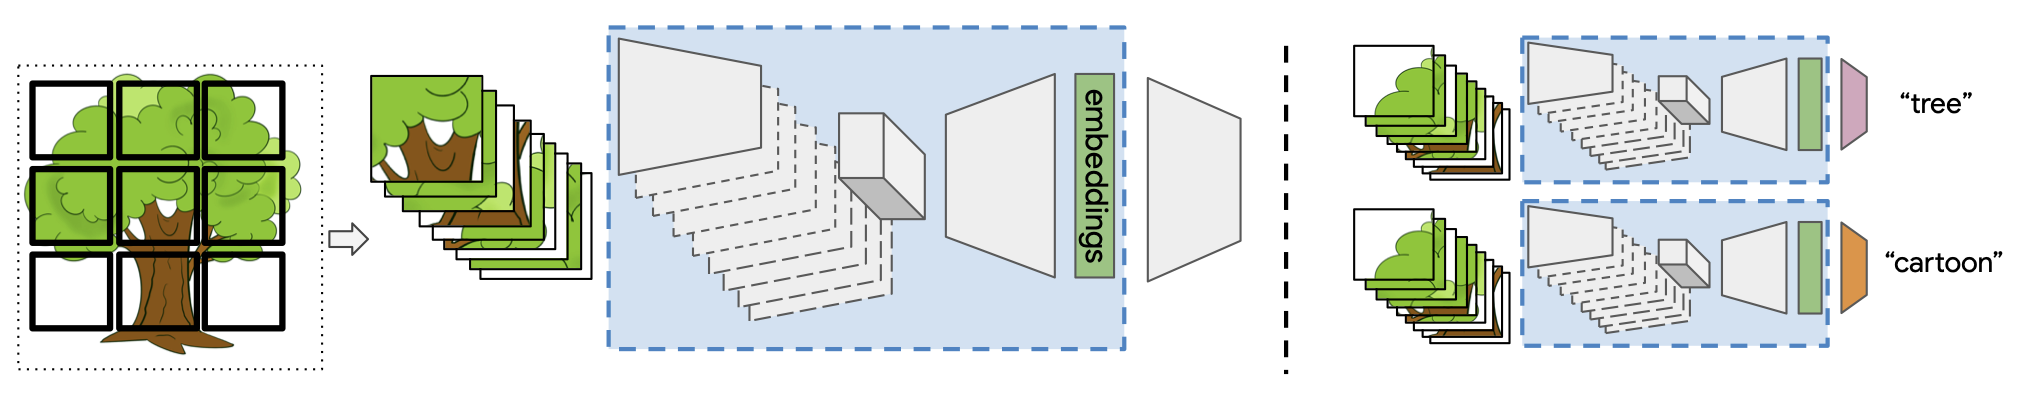
\includegraphics[width=\linewidth]{images/3/shuffle-to-learn}
 \caption{A self-supervised learning approach using shuffling image tiles as a pretext task presented by \citet{carr2021shuffle}. The trained feature encoder learns to extract relevant features and its parameters are transferred to a model trained to perform the downstream task.}
 \label{fig:ssl-pretext}
\end{figure}

Recently, a more common approach to SSL is \textbf{contrastive learning}.
This approach focuses on training the encoder to minimize the distance between feature vectors of similar (or positive) examples, while maximizing the distance between dissimilar (or negative) examples. Positive examples are generated in an unsupervised manner, often by applying random augmentations to an image to create two variants. The goal is for the feature vectors of these variants to be closely aligned. Notable implementations of contrastive learning include SimCLR \cite{chenSimpleFrameworkContrastive2020} and MoCo \cite{he2019moco}.

\section{Synthetic Data}

The data efficiency methods we've discussed so far revolve around pre-training networks with unlabeled or similar data. An alternative strategy involves generating synthetic data that mimics the target distribution. There are various techniques for this, each offering different levels of complexity and generation quality. A straightforward and commonly used method for expanding dataset size is \textbf{data augmentation}.

\textbf{Data augmentation} refers to the application of random transformations to input images, thereby artificially increasing their diversity. These transformations can be simple ones such as adjusting brightness or contrast, flipping the image horizontally, or more intricate, involving complex random deformations of the image. Generally the choice of transformations is governed by domain knowledge --- the network is forced to disregard transformations that we know it should be invariant to. Data augmentation is a standard practice in segmentation models, often employed alongside other data efficiency techniques. However, its implementation typically relies on simple deformation or transformation methods, which limits its capacity to create truly diverse samples.

Recently, the field of deep learning-based image generation, especially generative adversarial networks and diffusion models, have sparked a large interest in generating synthetic medical images. \textbf{Generative adversarial networks} \cite{goodfellowGenerativeAdversarialNetworks2014} consist of two neural networks, a generator and a discriminator, that are trained simultaneously. The generator creates synthetic images intended to be indistinguishable from real images, while the discriminator learns to differentiate between the two. The process continues until the generator produces images so convincing that the discriminator cannot easily distinguish them from real images. This technique has been particularly effective in generating realistic medical images for the purpose of data augmentation \cite{shinMedicalImageSynthesis2018}.

Diffusion models \cite{ho2020denoising}, a more recent development in the field of generative models, offer an alternative approach to image generation. These models, inspired by the physical process of diffusion, work by gradually adding noise to an image and then learning to reverse this process. The end result is the generation of new images by reversing the noise addition process from a randomly sampled noise distribution. Diffusion models have been shown to generate high-quality images that can be particularly useful in medical imaging contexts \cite{khaderDenoisingDiffusionProbabilistic2023}.


%\section{Regularization}
%
%As mentioned earlier, aside from getting new data, the easiest way to reduce the estimation error is by limiting the size of the function class our model optimizes. In a traditional machine learning approach, this would be done by hand-selecting a class of functions with a lower number of parameters and then training the model. In deep learning, however, this approach is usually replaced with regularization, where the parameters themselves are manipulated to simplify the model.\footnote{Often, any method of reducing the estimation error of a model is broadly termed as regularization.} Instead of selecting the number of parameters, we can penalize the network for the complexity and size of parameters. In other words, the loss function between a predicted model output $y_{pred}$ and a ground-truth label $y$ has the form:
%
%\begin{equation}
%	L(\theta; y_{pred}, y) = L_{seg}(\theta; y_{pred}, y) + \alpha\Omega(\theta)
%\end{equation}
%
%where $L_{seg}$ is the segmentation loss function while $\Omega(\theta)$ is a parameter norm penalty, i.e. a measure of the complexity of the model \cite{goodfellowDeepLearning2016}. As we increase $\alpha$, the strength of the regularization increases and the loss is more impacted by the complexity of the model. As the network is being trained, it will seek to both reduce $\Omega(\theta)$ as well as $L_{seg}$, leading to a more constrained model.
%
%A commonly used parameter norm penalty is the $L^2$ regularization, also known as \textbf{weight decay} in deep learning contexts. Assuming $\theta$ consists of a set of weights $w, \lvert w \rvert = n$ and biases $b$, the $L^2$ norm is defined as $\Omega(w) = \frac{1}{2}\sqrt{(w_1^2 + w_2^2 + \cdots + w_n^2)}$. In other words, the network is exponentially penalized for moving weights away from zero. This regularisation, in effect, forces the network to use fewer parameters.

\subsection{Conclusion}

As we have seen, there are a number of approaches to increasing the data efficiency of neural network-based segmentation of medical images. This thesis focuses on using regularisation by transforming the input data in such a way as to allow the network to use fewer parameters to achieve its segmentation task. We do so by combining predictions of neural networks with more traditional approaches from image processing and data augmentation. In the next chapter, we will introduce this idea and some specific applications.

%	\subsection{Leveraging Inductive Bias}
%	
%The core of achieving data and label efficiency is in manipulating the \textbf{inductive bias} of a model. If we are trying to approximate functions, we quickly run into a problem --- for any given set of finite points, we can find an infinite set of functions that can correctly approximate those points. Thus, we need to constrain the space of possible functions in some way. In the previous section, we assumed our functions were polynomial with a fixed number of degrees. That is an inductive bias --- we have biased our model to only consider polynomial relationships between the inputs and the labels.
%
%We can use inductive bias to our advantage. With a more constrained function space, the model can more easily converge to an optimal set of parameters. We have observed this effect in Figure \figref{fig:reg-deg-2}, where the 1 and 2-degree polynomials are able to closely fit the underlying function even with a few datapoints.
%
%We can also extend this to CNN architectures. Simply by using convolutions are their fundamental operation, a CNN has beneficial inductive biases for processing images. \todo{todo}
%	
%	\subsection{Transforming the Data}
	
%\section{Model-guided Transformations}

% todo in the book he mentions different feature representation
% 25.2 Feature Manipulation and Normalization

%When segmenting liver tumors in CT image, an expert, given a voxel location and image, can map each location to a probability of encountering a liver tumor on that image. They do so based on experience, intuition, and complex models of the real world including anatomy, pathology, biological processes of cancerous cell multiplication, understanding of how different vascular systems propagate contrast to cancerous and normal cells, etc. It is computationally infeasible to model these processes directly, so instead we opt for sampling a set of CT images and approximating the underlying processes as a continuous function.
%
%The sampled points are in the form of $(I(A), M(A))$ i.e. an image and segmentation map pair, as labeled by an expert. If we consider the image and segmentation map to be high-dimensional vectors, we can think of both as existing in a high-dimensional space.


%At their core, neural networks are function approximators. Every voxel in a CT scan contains either normal tissue or a liver tumor. Cancerous cells multiply and grow according to biological processes and are thus localized in specific areas. Because the cancerous cells are supplied with blood by the hepatic artery, an injected contrast reaches them sooner than normal cells, causing them to appear brighter in the image. These are just a few of infinitely many processes that govern the true probability of a voxel containing cancerous tissue. All of these processes together form an exceedingly complex function that maps a voxel its true probability of containing cancerous tissue. The goal of a segmentation network is to approximate this natural function using a statistical model. 
%
%We may imagine a CT scan as a point that lies in a high-dimensional space, where each voxel value is one dimension of the point.
%
%
%In image segmentation, this 
%
%At their core, neural networks aim to replicate natural phenomena. Somewhere in the real world, there exists a natural process producing measurable changes. Cancerous liver cells receive their blood supply from the hepatic artery, while normal liver cells are supplied mostly by the portal vein. During a CT with contrast, the injected contrast enters the hepatic arterial system first and travels to the liver cells making them briefly appear brighter than surrounding normal cells. This is a physical process that produces a single measurement --- a CT image. We can collect many such images to form a liver tumor segmentation dataset. Given this dataset, we can task a neural network to approximate 
%
%
%At their core, neural networks approximate a function given a set of data points. The goal of the research community is that this approximate function is as close as possible to a real natural phen
%
%The ultimate goal of any machine learning researcher is to improve the accuracy of a model under some set of conditions. The conditions that impact the accuracy of neural networks be broadly classified into three groups: model design, training procedure, and data. These conditions have a dynamic interplay. The most reliable way to increase performance is by getting more and better quality data. Good is a necessary condition



% capacity -- complexity -- sample size dependency
% inductive bias
% other methods (check notes)

% https://www.frontiersin.org/articles/10.3389/fncom.2022.760085/full

% https://www.cs.huji.ac.il/%7Eshais/UnderstandingMachineLearning/understanding-machine-learning-theory-algorithms.pdf#page=36
%on the algorithm being used. It only depends on the distribution D and on the hypothesis class H. Therefore, if the approximation error is large, it will not help us to enlarge the training set size, and it also does not make sense to reduce the hypothesis class. What can be beneficial in this case is to enlarge the hypothesis class or completely change it (if we have some alternative prior knowledge in the form of a different hypothesis class). We can also consider applying the same hypothesis class but on a different feature representation of the data (see Chapter 25).
%The estimation error of the class does depend on the sample size. Therefore, if we have a large estimation error we can make an effort to obtain more training examples. We can also consider reducing the hypothesis class. However, it doesn’t make sense to enlarge the hypothesis class in that case.

% The approximation error of the class does not depend on the sample size or on the algorithm being used. It only depends on the distribution D and on the hypothesis class H. Therefore, if the approximation error is large, it will not help us to enlarge the training set size, and it also does not make sense to reduce the hypothesis class. What can be beneficial in this case is to enlarge the hypothesis class or completely change it (if we have some alternative prior knowledge in the form of a different hypothesis class). We can also consider applying the same hypothesis class but on a different feature representation of the data (see Chapter 25). --- seems useful
% The estimation error of the class does depend on the sample size. Therefore, if we have a large estimation error we can make an effort to obtain more training examples. We can also consider reducing the hypothesis class. However, it doesn’t make sense to enlarge the hypothesis class in that case.
